%%%%%%%%%%%%%%%%%%%%%%%%%%%%%%%%%%%%%%%%%%%%%%%%%%%%%%%%%%%%%%%%%%%%%%%%%%%%%%%%
%2345678901234567890123456789012345678901234567890123456789012345678901234567890
%        1         2         3         4         5         6         7         8

\documentclass[letterpaper, 10 pt, conference]{ieeeconf}  % Comment this line out

 

% if you need a4paper
%\documentclass[a4paper, 10pt, conference]{ieeeconf}      % Use this line for a4
                                                          % paper

\IEEEoverridecommandlockouts                              % This command is only
                                                          % needed if you want to
                                                          % use the \thanks command
\overrideIEEEmargins
% See the \addtolength command later in the file to balance the column lengths
% on the last page of the document



% The following packages can be found on http:\\www.ctan.org
%\usepackage{graphics} % for pdf, bitmapped graphics files
%\usepackage{epsfig} % for postscript graphics files
%\usepackage{mathptmx} % assumes new font selection scheme installed
%\usepackage{times} % assumes new font selection scheme installed
%\usepackage{amsmath} % assumes amsmath package installed
%\usepackage{amssymb}  % assumes amsmath package installed
%\usepackage{natbib}

% packages actually used for this report
\usepackage{amsmath, amsfonts, amssymb}
\usepackage{graphicx}
\usepackage{tikz}
\usetikzlibrary{matrix}

% some custom commands
\newcommand{\flow}{\operatorname{flow}}
\newcommand{\txvalue}{\operatorname{value}}

\title{\LARGE \bf
Analysis of the Bitcoin Transaction Graph
}

\author{Devanshu Agrawal, James Cate, Kevin Gardner, and  Chris Shurtleff% <-this % stops a space
%\thanks{*This work was not supported by any organization}% <-this % stops a space
}


\begin{document}



\maketitle
\thispagestyle{empty}
\pagestyle{empty}


%%%%%%%%%%%%%%%%%%%%%%%%%%%%%%%%%%%%%%%%%%%%%%%%%%%%%%%%%%%%%%%%%%%%%%%%%%%%%%%%
\begin{abstract}
Bitcoin is a popular cryptocurrency based on blockchain technology. The exchange of bitcoins between addresses can be modeled as a directed graph. Bitcoin transactions themselves make reference to one another and therefore exhibit a graph structure as well. We analyzed various attributes of the bitcoin transaction graph including degree distribution and their dynamics over time. We also introduced the notion of bitcoin flow and used it to probe the structure of the graph. We found that small samples of the bitcoin transaction graph are scale-free and carry attributes that are very stable over both time and scale.
\end{abstract}


%%%%%%%%%%%%%%%%%%%%%%%%%%%%%%%%%%%%%%%%%%%%%%%%%%%%%%%%%%%%%%%%%%%%%%%%%%%%%%%%
\section{Introduction}

Bitcoin is a popular cryptocurrency based on a white paper by Nakamoto Satoshi \cite{sat2008}. The bitcoin protocol enables the cryptographically secure transfer of bitcoins through the use of a public ledger known as the blockchain. The bitcoin blockchain consists of a series of transactions collected and verified by independent users known colloquially as 'bitcoin miners'. The blockchain thus consists of a publicly available ledger of every single transfer of bitcoin to date. This paper seeks to model the bitcoin blockchain as two separate graphs to gain insights on how people are using bitcoin, and proposes a method to measure the relationship between two transactions.

Previous researchers have used statistical analysis of the bitcoin transactions graph and its features to develop insights into the behavior of users and transactions. For example, it was found that most large transactions in 2012 could be traced back to one single transaction in 2010 and that the subgraph of such large transactions exhibited peculiar features-- perhaps an attempt to conceal or obscure suspicious activity \cite{ron2012}. This example motivates the idea that even though bitcoin transactions are in principle anonymous, it could still be possible to detect suspicious activity by revealing anomalous structures in the bitcoin transactions graph. For instance, it has been shown that certain local features in the bitcoin transactions graph (e.g., degree and clustering coefficient) can allow us to cluster users and transactions and thus to detect suspicious outliers that should be flagged for further investigation \cite{pham2016, zambre2013}.

The core structure of bitcoin transactions is that they make reference to previous transactions and therefore allow bitcoins to be traced. We believe that local feature extraction from the bitcoin transactions graph fails to fully capture this essential structure; for our project, we compare instead transactions based on the flow of bitcoins common to both transactions.


\section{Theoretical Concepts}

\subsection{Bitcoin Address Graph}

A \emph{bitcoin address graph} (BAG) is a directed multigraph whose nodes represent distinct bitcoin addresses and whose arcs represent not necessarily distinct bitcoin transactions. By ``multigraph'', we mean that multiple arcs between the same pair of nodes are permitted. We consider a hypothetical example of a BAG that illustrates many important concepts (Figure \ref{bag}). In this example, nodes $A$-$F$ represent distinct bitcoin addresses. Node ``Base'' represents the source of all newly mined bitcoins.

\begin{figure}
\centering
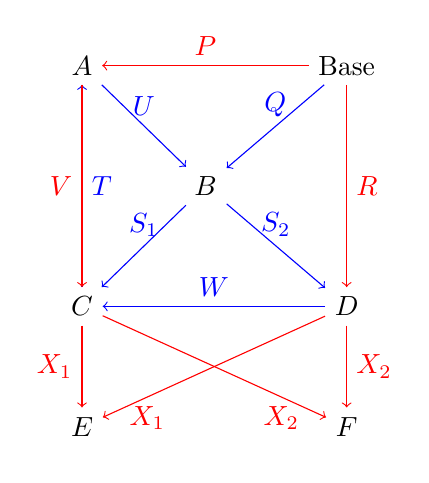
\begin{tikzpicture}[every node/.style={midway}]
\matrix[column sep={3em}, row sep={3em}] at (0,0)
{
\node(a){$A$}; & & \node(base){Base}; \\
& \node(b){$B$}; & \\
\node(c){$C$}; & & \node(d){$D$}; \\
\node(e){$E$}; & & \node(f){$F$}; \\
};
\draw[->, red] (base)--(a) node[anchor=south]{$P$};
\draw[->, blue] (base)--(b) node[anchor=south]{$Q$};
\draw[->, red] (base)--(d) node[anchor=west]{$R$};
\draw[->, blue] (b)--(c) node[anchor=south]{$S_1$};
\draw[->, blue] (b)--(d) node[anchor=south]{$S_2$};
\draw[->, blue] (d)--(c) node[anchor=south]{$W$};
\draw[->, blue] (c)--(a) node[anchor=west]{$T$};
\draw[->, blue] (a)--(b) node[anchor=south]{$U$};
\draw[->, red] (a)--(c) node[anchor=east]{$V$};
\draw[->, red] (c)--(e) node[anchor=east]{$X_1$};
\draw[->, red] (c)--(f) node[anchor=north, pos=0.8]{$X_2$};
\draw[->, red] (d)--(f) node[anchor=west]{$X_2$};
\draw[->, red] (d)--(e) node[anchor=north, pos=0.8]{$X_1$};
\end{tikzpicture}
\caption{\label{bag} Hypothetical example of a BAG.}
\end{figure}

Let us walk through the transactions depicted in the example BAG. Transactions $P$, $Q$, and $R$ are coinbase transactions so that $A$, $B$, and $D$ are successful bitcoin miners. In transaction $S$, address $B$ sends bitcoins to two addresses $C$ and $D$ along two \emph{out-branches} $S_1$ and $S_2$. This illustrates that a single transaction can have multiple out-branches. In transaction $T$, address $C$ sends bitcoins to address $A$, which in turn sends bitcoins back to $B$ in transaction $U$. Transactions $S$ (out-branch $S_1$), $T$, and $U$ therefore form a (directed) cycle among addresses $B$, $C$, and $A$. In fact, we will see later that address $B$ receives exactly the same bitcoins from $A$ that it had sent to $C$.

In transactions $V$ and $W$, address $C$ receives bitcoins from $A$ and $D$ respectively. Observe that address $C$ both sends (transaction $T$) and recieves (transaction $V$) bitcoins from $A$. This is one example of how multiple arcs are permitted between the same pair of nodes. We could also have multiple arcs with the same orientation; this would indicate that one address sent bitcoins to another address through multiple transactions.

We now turn our attention to transaction $X$. This transaction has two sending addresses $C$ and $D$ and two receiving addresses $E$ and $F$. But despite there being four arcs depicting the transaction, there are only two out-branches $X_1$ and $X_2$. More precisely, there is one out-branch per receiving address. This is because a bitcoin transaction only records the bitcoin value sent by each sending address and the bitcoin value received by each receiving address; the transaction does not record the specific breakdown (i.e., the value that each sending address sends to each receiving address) as it plays no role in the bitcoin technology. Transaction $X$ illustrates that a transaction can in general have multiple sending addresses and receiving addresses.

Although it is not depicted in the example BAG, every arc can be weighted by a bitcoin value. For example, a weight on transaction $P$ would indicate the number of bitcoins that address $A$ mined with that one coin base transaction, and a weight on transaction $S_2$ would be the number of bitcoins that address $B$ sent to $D$. In the case of transaction $X$, the explicit bitcoin values for the four arcs are not recorded. But we do know the values that $C$ and $D$ send and the values that $E$ and $F$ recieve. From these values we can estimate the value that address $E$ receives from $C$ as
\begin{align*}
&\quad [\mbox{value E receives from C}] \\
&= [\mbox{value E receives}]\left(\frac{[\mbox{value C sends}]}{\mbox{ value C and Dsend}]}\right).
\end{align*}
We can estimate the values on the other three arcs analogously.


\subsection{Transaction Graph}

Every bitcoin transaction is said to ``hold'' a bitcoin value. This is simply the weight of a transaction in a BAG. A bitcoin address is said to ``control'' all the transactions from which it received bitcoins. For instance in the example BAG, address $C$ controls transactions $S_1$, $T$, and $W$.

In order for an address to send bitcoins to another address, it must \emph{spend} some number of its controlled transactions. The value of a transaction must be spent in its entirety and can only be spent once. The total value of the controlled transactions to be spent must be at least the value that is to be sent to the second address. Formally, if some address $A$ spends transactions $I$, $J$, $K$, \ldots in order to perform a transaction $T$, then we say that $I$, $J$, $K$, \ldots are the \emph{input transactions} or simply \emph{inputs} of $T$.

Recall the example BAG. In the depiction, two adjacent arcs of opposite orientation are of the same color if one is an input transaction of the other. For instance, address $D$ controls transactions $R$ and $S_2$. Address $D$ spends $R$ in order to perform transaction $W$ and send bitcoins to $C$. We could say that $D$ transferred ownership of the bitcoins held in $R$ to $C$ via transaction $W$. Similarly, $D$ spends $S_2$ in order to partake in transaction $X$ and send bitcoins to $E$ and $F$.

The requirement that every transaction (except coinbase transactions) refer to previous transactions as inputs defines a structure that allows the flow of bitcoins to be traced. Recall the cycle formed by addresses $A$, $B$, and$C$ in the example BAG. The three arcs $S_1$, $T$, and $U$ are of the same color (blue). This means that $C$ spent $S_1$ to perform $T$, and $A$ spent $T$ to perform $U$. It is for this reason that we could say that the bitcoins sent to $B$ by $A$ are exactly the same ones that $B$ sent to $C$. Suppose instead that $A$ spent $P$ to perform $U$. Then the bitcoins that $B$ sent to $C$ would not return to $B$.

Consider as another example the bitcoins owned by $E$ and $F$. We see from the depicted example BAG that these bitcoins once belonged to $A$, $C$, and $D$ but never to $B$. This is how the structure of bitcoin transactions allows for bitcoin tracking.

The reference of a transaction to previous transactions means that the notion of ``adjacent'' transactions is well-defined. A \emph{bitcoin transaction graph} (BTG) is a directed graph whose nodes represent distinct bitcoin transactions and whose arcs represent references to input transactions. More precisely, we draw an arc from transaction $T$ to transaction $U$ if $T$ is an input of $U$; i.e., the parent nodes of a transaction are precisely its input transactions. We construct the BTG for the example BAG (Figure \ref{btg}). Node ``Base'' is a construct that represents the input of all coin base transactions and is the only root node in the BTG. 

\begin{figure}
\centering
\begin{tikzpicture}[every node/.style={midway}]
\matrix[column sep={3em}, row sep={3em}] at (0,0)
{
\node(u){$U$}; & & \\
\node(t){$T$}; & & \node(w){$W$}; \\
& \node(s){$S$}; & \\
& \node(q){$Q$}; & \\
& \node(base){Base}; & \\
\node(p){$P$}; & & \node(r){$R$}; \\
\node(v){$V$}; & & \node(x){$X$}; \\
};
\draw[->, red] (base)--(p);
\draw[->, red] (base)--(r);
\draw[->, red] (p)--(v);
\draw[->, red] (r)--(x);
\draw[->, red] (v)--(x);
\draw[->, blue] (base)--(q);
\draw[->, blue] (q)--(s);
\draw[->, blue] (s)--(t);
\draw[->, blue] (s)--(w);
\draw[->, blue] (t)--(u);
\end{tikzpicture}
\caption{\label{btg} Example BTG constructed from the example BAG shown in Figure \ref{bag}}.
\end{figure}

Notice in the example BTG that out-branches of transactions are not specified. Recall, for instance, that transaction $S$ had two out-branches. But in the BTG, we do not use separate nodes for out-branches $S_1$ and $S_2$ but instead only one node for the transaction $S$. This is because the purpose of the BTG (as we will see later) is to track bitcoin flow, and it turns out that not specifying out-branches leads to no ambiguities during bitcoin tracking. Another upside of this simplification is that the BTG is a simple directed graph; i.e., there can be at most one arc between any pair of transactions.

Observe also that the BTG carries no cycles-- even though the corresponding BAG did. This is because no transaction can be an input for a transaction that has already occurred. We then see that the BTG is a directed acyclic graph (DAG) and therefore offers a concrete representation of the rich structure hidden in the BAG.

The structure of a DAG is natural for tracking flow. We see in the example BTG for instance that transaction $X$ has ancestors $V$, $R$, $P$ and ``Base''. But none of these ancestors was ever controlled by address $B$. Therefore, the bitcoins held in transaction $X$ (which belong to addresses $E$ and $F$) did not flow through address $B$. We give a more quantitative formulation of flow next.


\subsection{Tracking Bitcoin Flow}

The \emph{flow} to a transaction $T$ from a transaction $U$ -- denoted $\flow(T,U)$ is the fraction of bitcoins held in $T$ that were once held in $U$. We should think of $\flow(T,U)$ as the probability that a bitcoin held in $T$ was at some point held in $U$.

We consider a simple example. Let $U_1,U_2,\ldots,U_n$ be the inputs of a transaction $T$. Then,
\begin{equation} \label{eq1}
\flow(T,U_i) = \frac{\txvalue(U_i)}{\sum_{j=1}^n \txvalue(U_j)}.
\end{equation}
Equation \ref{eq1} lets us compute $\flow(T,U)$ for every arc $U\rightarrow T$ in a BTG. We assign these single-arc flows as probability weights to all arcs in the BTG.

Consider now a hypothetical BTG that is just a single path of transactions $[T_1,T_2,\ldots,T_n]$ where $T_{i+1}$ is the input of $T_i$. By properties of probability, the flow to the head of the path from its tail is
\begin{equation} \label{eq2}
\flow(T_1, T_n) = \prod_{i=1}^{n-1} \flow(T_i, T_{i+1}).
\end{equation}
We generalize this to more realistic topologies as follows: Suppose we wish to compute $\flow(T, U)$ for some transactions $T$ and $U$. We first construct a subgraph of the BTG induced on the nodes
\[ H = (\{T\}\cup\operatorname{ancestors}(T))\cap (\{U\}\cup\operatorname{descendents}(U)). \]
Every maximal path in H is necessarily a path from $U$ to $T$. Let $\mbox{Paths}$ be the set of all such paths in $H$. Then the flow to $T$ from $U$ is just the sum of flows over all paths:
\begin{equation} \label{eq3}
\flow(T, U) = \sum_{\mbox{path}\in\mbox{Paths}}\flow(T, U;\mbox{path}),
\end{equation}
where $\flow(T, U;\mbox{path})$ is the flow restricted along the path ``$\mbox{path}$'' computed using Equation \ref{eq2}.

There is a more efficient way to compute flow than Equation \ref{eq3}. Since the subgraph $H$ is a DAG (since it is a subgraph of a DAG), then its nodes can be partitioned into layers. Let $L_i$ be the set of all leaf nodes in $H_i$ where $H_1 = H$ and $H_{i+1} = H_i\setminus L_i$. Assuming $n$ layers $L_1,\ldots,L_n$, we have $L_1=\{T\}$ and $L_n=\{U\}$. Every transaction in $L_2$ is an input of $T$ so that we can calculate $\flow(T, V)$ using Equation \ref{eq1} for every $V\in L_2$. Computation of flow from transactions in higher layers follows by induction: Suppose $\flow(T, V)$ has been computed for every $V\in L_i$. Then for every $W\in L_{i+1}$, we have
\begin{equation} \label{eq4}
\flow(T, W) = \sum_{V\in\operatorname{children}(W)} \flow(T, V)\flow(V, W).
\end{equation}
Equation \ref{eq4} effectively lets us compute flows over all paths in $H$ in parallel. This recursive approach grants us the bonus that the intermediate flows to $T$ from all of its ancestors up to $U$ are calculated. In fact, the evaluation of $\flow(T, \mbox{Base})$ effectively calculates $\flow(T, V)$ for every $V\in\operatorname{ancestors}(T)$.

The above formulation lets us compute flow between transactions. It is also possible to compute flow between addresses. The bitcoin flow to an address $A$ from an address $B$ is an aggregation of flows to each transaction that $A$ controls from each transaction that $B$ performs. The problem is that these flows are not necessarily independent (i.e., overlap) and therefore cannot simply be summed. Instead, significant adjustments must be made to ensure that no fraction of flow is over-counted. This leads to significant combinatorial challenges, and so we save computation of flow between addresses for future work.


\section{Methods and Procedures}

We implemented methods to gather data and construct graphs for both the BAG and BTG. But we were unable to complete data collection and analysis for the BAG. We therefore only discuss our methods for the construction of the BTG.

\subsection{Data Collection}

We used the blockchain.info API to retrieve data. The API accepts as argument a block hash and returns the data for the appropriate block in JSON format. The block JSON contains a field ``tx'' that lists JSON dictionaries for all transactions in the block. Each transaction JSON contains a field ``inputs'' that lists all input transactions. The relevant information in each input is provided by the ``prev\_out'' field, which contains the input address, input value, input transaction hash, and input transaction index. The transaction index is specific to blockchain.info but has the advantage that it is significantly smaller in size as compared to the transaction hash.

We implemented python scripts to automate data collection and parsing. The API accepts as argument a seed block hash and the number of blocks for which data is desired. The API retrieves the JSON for the seed block and parses the transaction index, input transaction indices, and input values for every transaction in the block. The block JSON contains a field ``prev\_block'' that provides the hash of the preceding block in the block chain. Our API then retrieves and parses data for this preceding block and iterates data gathering in this way for the number of blocks specified.

The parsed data is written to a CSV file with the following attributes: Input transaction index, output transaction index, input value, and flow probability. Each transaction JSON that is parsed can result in multiple lines written to the CSV file-- one line per input transaction. The flow probability refers to the flow to the output transaction from the input and is calculated on the fly using Equation \ref{eq1}.

Coinbase transactions are something of a special case. The JSON of a coinbase transaction does not contain a ``prev\_out'' field. We define the input transaction of a coinbase transaction as the integer $-1$ (we do not use ``Base'' as we want all transaction indices to be integer type), and we calculate the input value as the sum of all output values; the output value information is contained in the ``out'' field of the transaction JSON.

We log all block hashes for which data is collected. The demarcation of blocks in the data CSV file is defined by the coinbase transactions (rows whose input transaction index column contains $-1$) as the first transaction in every block is a coinbase transaction.


\subsection{Graph Construction}

We implemented the BAG and BTG as subclasses of the ``DiGraph'' class  from the NetworkX python module. We discuss only the BTG. The BTG class contains a method to build the graph given a CSV file of transaction data in the format described above. A node is instantiated for every unique transaction index in the CSV file, and every node is labeled with its transaction index. Each line of the CSV file defines an arc from input to output transaction weighted by input value and flow probability. The BTG class also contains a method that calculates flow for any pair of transactions in the BTG or alternatively the flows to a transaction from all of its ancestors. The BTG class also inherits all attributes and methods from the DiGraph so that methods for extracting information such as degree distribution are available out of the box.


\section{Experiments}

We originally collected data for 1000-block samples for 23 months: May-December 2015, May-December 2016, and May-November 2017. For each month, we selected a hash for a block that was confirmed near the middle of the month and gathered data for the 1000 blocks leading up to the selected seed block. Data collection and storage were straightforward. But construction of the BTG on each 1000-block sample proved computationally infeasible given our resources. We therefore cut our sample size down to 100 blocks per month.

\subsection{Distributions}

We used the CSV data generated from each 100-block sample to construct a BTG. We recorded the in-degree distribution, out-degree distribution, and component size distribution for each graph. We also collected flow data for each graph as follows: In a 100-block BTG, we found the head node of the longest path-- call it $T$. We took the subgraph generated by $T$ and its ancestors and organized it into layers. We took only the first 100 layers including $T$. Call the resulting subgraph $H$. We recorded the distance of each $V\in H$ from $T$ (e.g., a node in the $i$th layer is a distance $i-1$ from $T$) as well as the flow $\flow(T, V)$. We recorded this data as distance vs. flow.

Here we present the in-degree distribution, out-degree distribution, and component size distribution only for the 100-block sample collected from mid-November 2017; the distributions for all other months were similar. The BTG for November 2017 has order $415759$.

The in-degree distribution strictly decreases (Figure \ref{in-degree-distro}). Most transactions have only one input. The in-degree distribution is approximately linear on a log-log scale. This means that the in-degree follows a power-law distribution and therefore that the BTG is scale-free. A \emph{scale-free graph} is a graph that exhibits features at every scale. Many large networks such as social networks are known to be scale-free. We are not the first to suggest that the BTG is scale-free-- e.g., \cite{kondor2014rich}. But the fact that we were able to reproduce this result with only a 100-block sample -- less than a day's worth of blocks -- means that our sample -- although small -- is large enough to capture some nontrivial structure of the entire BTG.

\begin{figure}
\centering
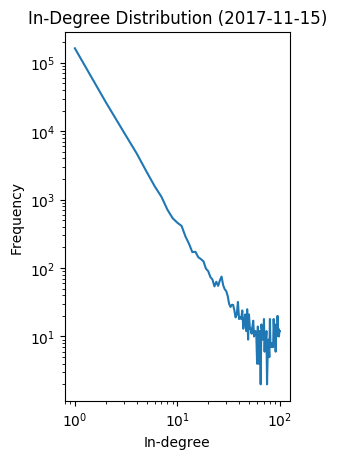
\includegraphics[width=3in]{Plots/In_degree_distros/2017-11-15.png}
\caption{\label{in-degree-distro} Plot of the in-degree distribution of the BTG constructed from a 100-block sample from November 2017.}
\end{figure}

The out-degree distribution is similar to the in-degree distribution (Figure \ref{out-degree-distro}). Most transactions have only one out-branch-- i.e., one receiving address. The distribution is also approximately linear on a log-log scale so that the out-degree follows a power law distribution. This supports the hypothesis that the BTG is scale-free. We observe, however, that the plot is not as linear as the plot of the in-degree distribution. We believe this is due to sampling bias: The transaction JSONs that we parse contain complete information about input transactions. Thus, the inclusion of additional blocks would not change the in-degree of nodes. But the out-branches of a transaction are included in our data only if they are found to be inputs of other transactions; this depends on the number of blocks we include in our sample. We expect the out-degree distribution to become more linear on a log-log scale as we add more blocks to our sample.

\begin{figure}
\centering
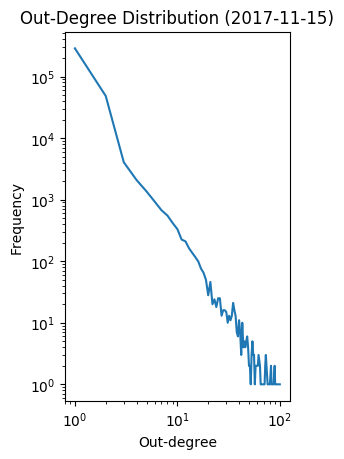
\includegraphics[width=3in]{Plots/Out_degree_distros/2017-11-15.png}
\caption{\label{out-degree-distro} Plot of the out-degree distribution of the BTG constructed from a 100-block sample from November 2017.}
\end{figure}

The component size distribution is approximately linear on a log-log scale as well (Figure \ref{comp-distro}). Most components are a single transaction with a single input (two nodes). This suggests that the BTG is highly disconnected. Nevertheless, the largest component contains $309704$ nodes-- about $74.5\%$ the size of the entire BTG for the 100-block sample. In theory, the BTG for the blockchain is connected since the value of every transaction can be traced back to the universal ancestor ``Base''. We therefore believe that the observed disconnectedness is due to sampling. The result that sampling ``shatters'' the BTG so that it has a very large number of small components suggests that the BTG is sparse. If this is true, then this property may enhance network security as tracking bitcoin flow would be more difficult.

\begin{figure}
\centering
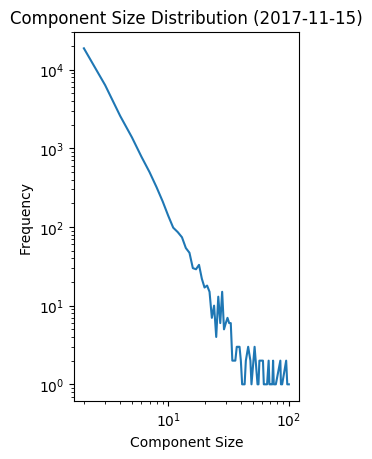
\includegraphics[width=3in]{Plots/Comp_distros/2017-11-15.png}
\caption{\label{comp-distro} Plot of the component size distribution of the BTG constructed from a 100-block sample from November 2017.}
\end{figure}

In addition to distributions of graph attributes, we collected distance vs. flow data as described at the beginning of this section. Unlike the distributions, we found the distance vs. flow data to vary significantly with time. We handpicked three examples for discussion (Figure \ref{distance-flow}). The flow for September 2016 maintains a value of $1$ over the entire range of distances shown. This suggests that the subgraph $H$ on which the flow was computed is a path of single-input transactions so that flow cannot diffuse. The flow for November 2017 exhibits a similar trend up to a distance of about $23$. But the flow drops to almost $0$ for larger distances. This suggests that the subgraph $H$ starts as a path of single-input transactions but bifurcates with one branch quickly ending at a root node (further input not available due to sampling) and another branch along which the flow is very small. The dynamics of flow for September 2016 and November 2017 are therefore very simple and again suggest that the BTG is sparse. The flow for September 2015, however, is more interesting. We observe multiple values of flow for the same values of distance. This suggests that the subgraph $H$ has numerous branches; i.e., transactions in $H$ have multiple inputs. This is an example of a more complex structure in the BTG and warrants further investigation in future work.

\begin{figure}
\centering
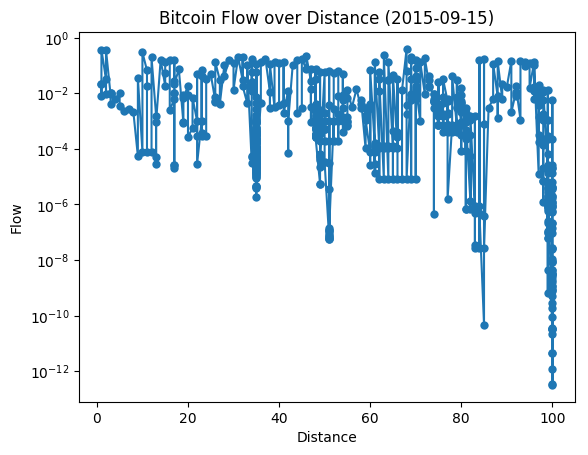
\includegraphics[width=3in]{Plots/Flow_distros/2015-09-15.png} \newline
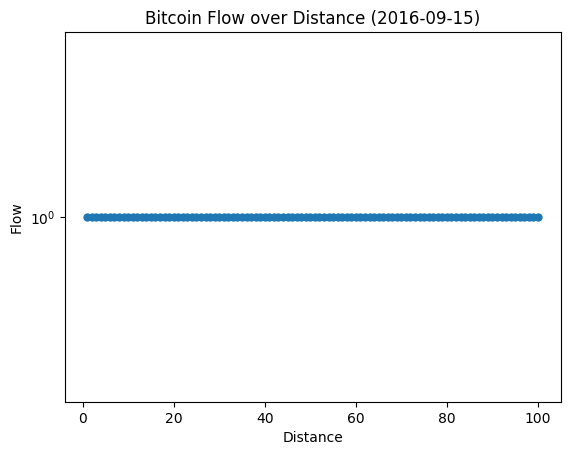
\includegraphics[width=3in]{Plots/Flow_distros/2016-09-15.png} \newline
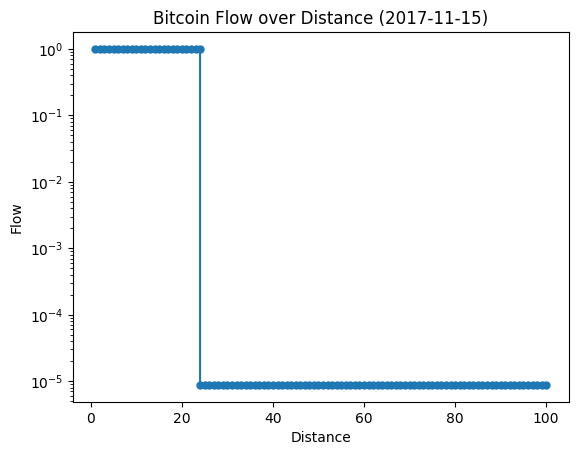
\includegraphics[width=3in]{Plots/Flow_distros/2017-11-15.png}
\caption{\label{distance-flow} Plots of flow to the head node of the longest path from its ancestors at various distances in the BTG constructed from 100-block samples for September 2015, September 2016, and November 2017.}
\end{figure}


\subsection{Trends over Time}

Here we present the trends of some graph attributes of the BTG over time (i.e., over the 23 months from which we drew 100-block samples).

The order of the BTG increases approximately linearly with time (Figure \ref{order}). This suggests that more transactions are being performed with time and thus indicates an increase in bitcoin activity.

\begin{figure}
\centering
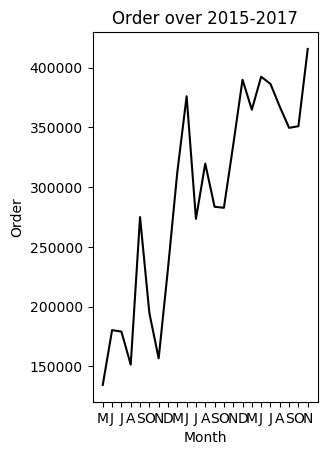
\includegraphics[width=3in]{Plots/Time/order.png}
\caption{\label{order} Plot of the order of the BTG constructed from 100-block samples over 23 months.}
\end{figure}

The in-degree, out-degree, and component size means and standard deviations are roughly constant with time (Figures \ref{in-degree}-\ref{comp}). This is remarkable as it indicates that our BTG has some stable properties despite its construction from such a small sample size of 100 blocks. The almost constant trends could establish a baseline against which anomalies could be detected-- if not in 2015-2017 then perhaps in the future.

\begin{figure}
\centering
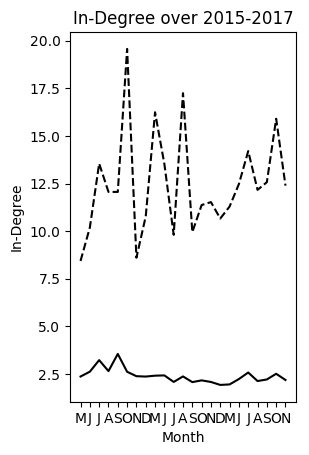
\includegraphics[width=3in]{Plots/Time/in_degree.png}
\caption{\label{in-degree} Plot of the mean in-degree (solid) and associated standard deviation (dashed) of the BTG constructed from 100-block samples over 23 months.}
\end{figure}

\begin{figure}
\centering
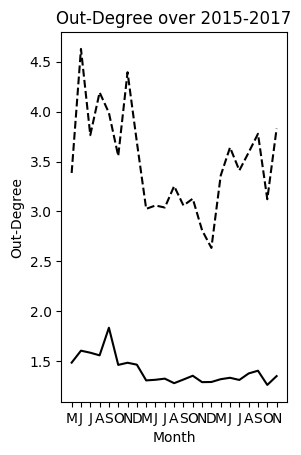
\includegraphics[width=3in]{Plots/Time/out_degree.png}
\caption{\label{out-degree} Plot of the mean out-degree (solid) and associated standard deviation (dashed) of the BTG constructed from 100-block samples over 23 months.}
\end{figure}

\begin{figure}
\centering
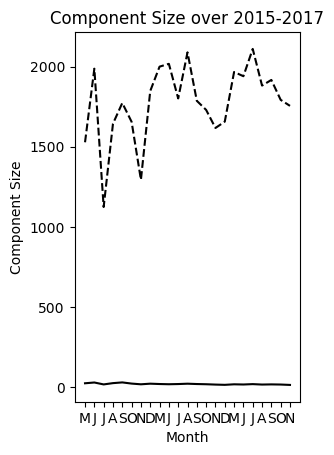
\includegraphics[width=3in]{Plots/Time/comp.png}
\caption{\label{comp} Plot of the mean component size (solid) and associated standard deviation (dashed) of the BTG constructed from 100-block samples over 23 months.}
\end{figure}

The flow mean and standard deviation is approximately constant through 2015 but exhibits erratic fluctuations afterwards (Figure \ref{flow}). We think the fluctuations are a result of instability in our model; recall that we calculated flow only to the head node $T$ of the longest path in the BTG. The fluctuations indicate drastic changes in the subgraph surrounding $T$ over time. In short, we believe the fluctuations to be noise.

\begin{figure}
\centering
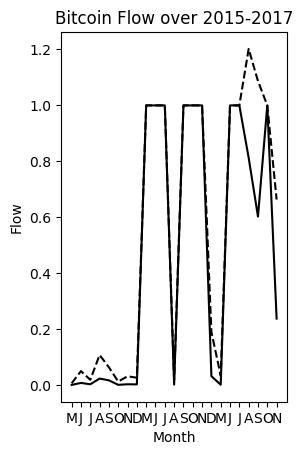
\includegraphics[width=3in]{Plots/Time/flow.png}
\caption{\label{flow} Plot of the mean flow (solid) and associated standard deviation (dashed) to the head node of the longest path in the BTG constructed from 100-block samples over 23 months.}
\end{figure}


\section{Discussion}

Bitcoin addresses are linked together through transactions that are themselves endowed with a rich topological structure. The BTG is an explicit representation of this topology. We found that the BTG is scale-free based only on 100-block samples. We also found that while most nodes in a 100-block BTG are contained in a single connected component, there are also many small components. This could simply be an artifact of a small sample size. But it could also point to the fragility of the BTG; the deletion or lack of inclusion of some transaction nodes ``shatters'' the connectivity of the graph. Indeed, suppose the BTG consists of several hubs that are weakly connected to one another but are all connected to the coin base. Then sampling could easily shatter the graph into a collection of isolated hubs.

We found that flow often  captures seemingly trivial structures in the BTG such as long paths of single-input transactions. But this reflects the fragility of the BTG and the simplicity of most transactions. But flow occasionally captures more complex behavior as in the case of the September 2015 sample. The reason for this behavior needs to be explored further.

We also observed that most basic graph attributes of the BTG do not significantly change over time despite a steady increase in order. This is remarkable as it means that the dynamics of the BTG are very stable. This stability could be used to establish a baseline against which anomalous behavior could be detected; any significant deviation from the baseline would warrant further investigation of a sample BTG.

We take the findings presented here only as motivation for deeper and more extensive investigations in the future. First, we would like to gather more evidence for the scale-freeness of the BTG; e.g., we would like to study the clustering coefficient distribution. Scale-freeness would imply the existence of large hubs of transactions that are themselves comprised of smaller hubs. We would like to identify these hubs. What are the large transactions that are central to the BTG, and which addresses are responsible for these transactions?

We would also like to include an ``unspent'' node in the BTG that would act as a universal sink for the graph. We would like to identify ``flow bottlenecks'' in the graph that suggest bitcoin hoarding.

We would also like to investigate the BAG. Our original plan was to compute flow on the BAG. This is an extension of flow on the BTG; we would have to compute the flow between every transaction controlled by the receiving address and every transaction performed by the sending address. This task proves to be a combinatorial challenge. We plan in the future to investigate strategies to overcome this hurdle. One idea would be to explore stochastic implementations of flow on the BAG-- e.g., markov chain simulations.

In addition to flow, we are also interested in gathering basic graph statistics on the BAG. Is the BAG scale-free as well? If so, then what are its hubs? Which addresses are critical to the connectivity of the BAG?

Finally, it is vital that we overcome the challenge of scalability. We seek a methodology that would let us scale our experiments to larger block samples and ideally the entire blockchain. The use of graph databases is a possibility. We believe that real insights into the structure of bitcoin exchange will emerge only at these larger scales.


\bibliographystyle{plainnat}
\bibliography{references}

\begin{figure}
\centering
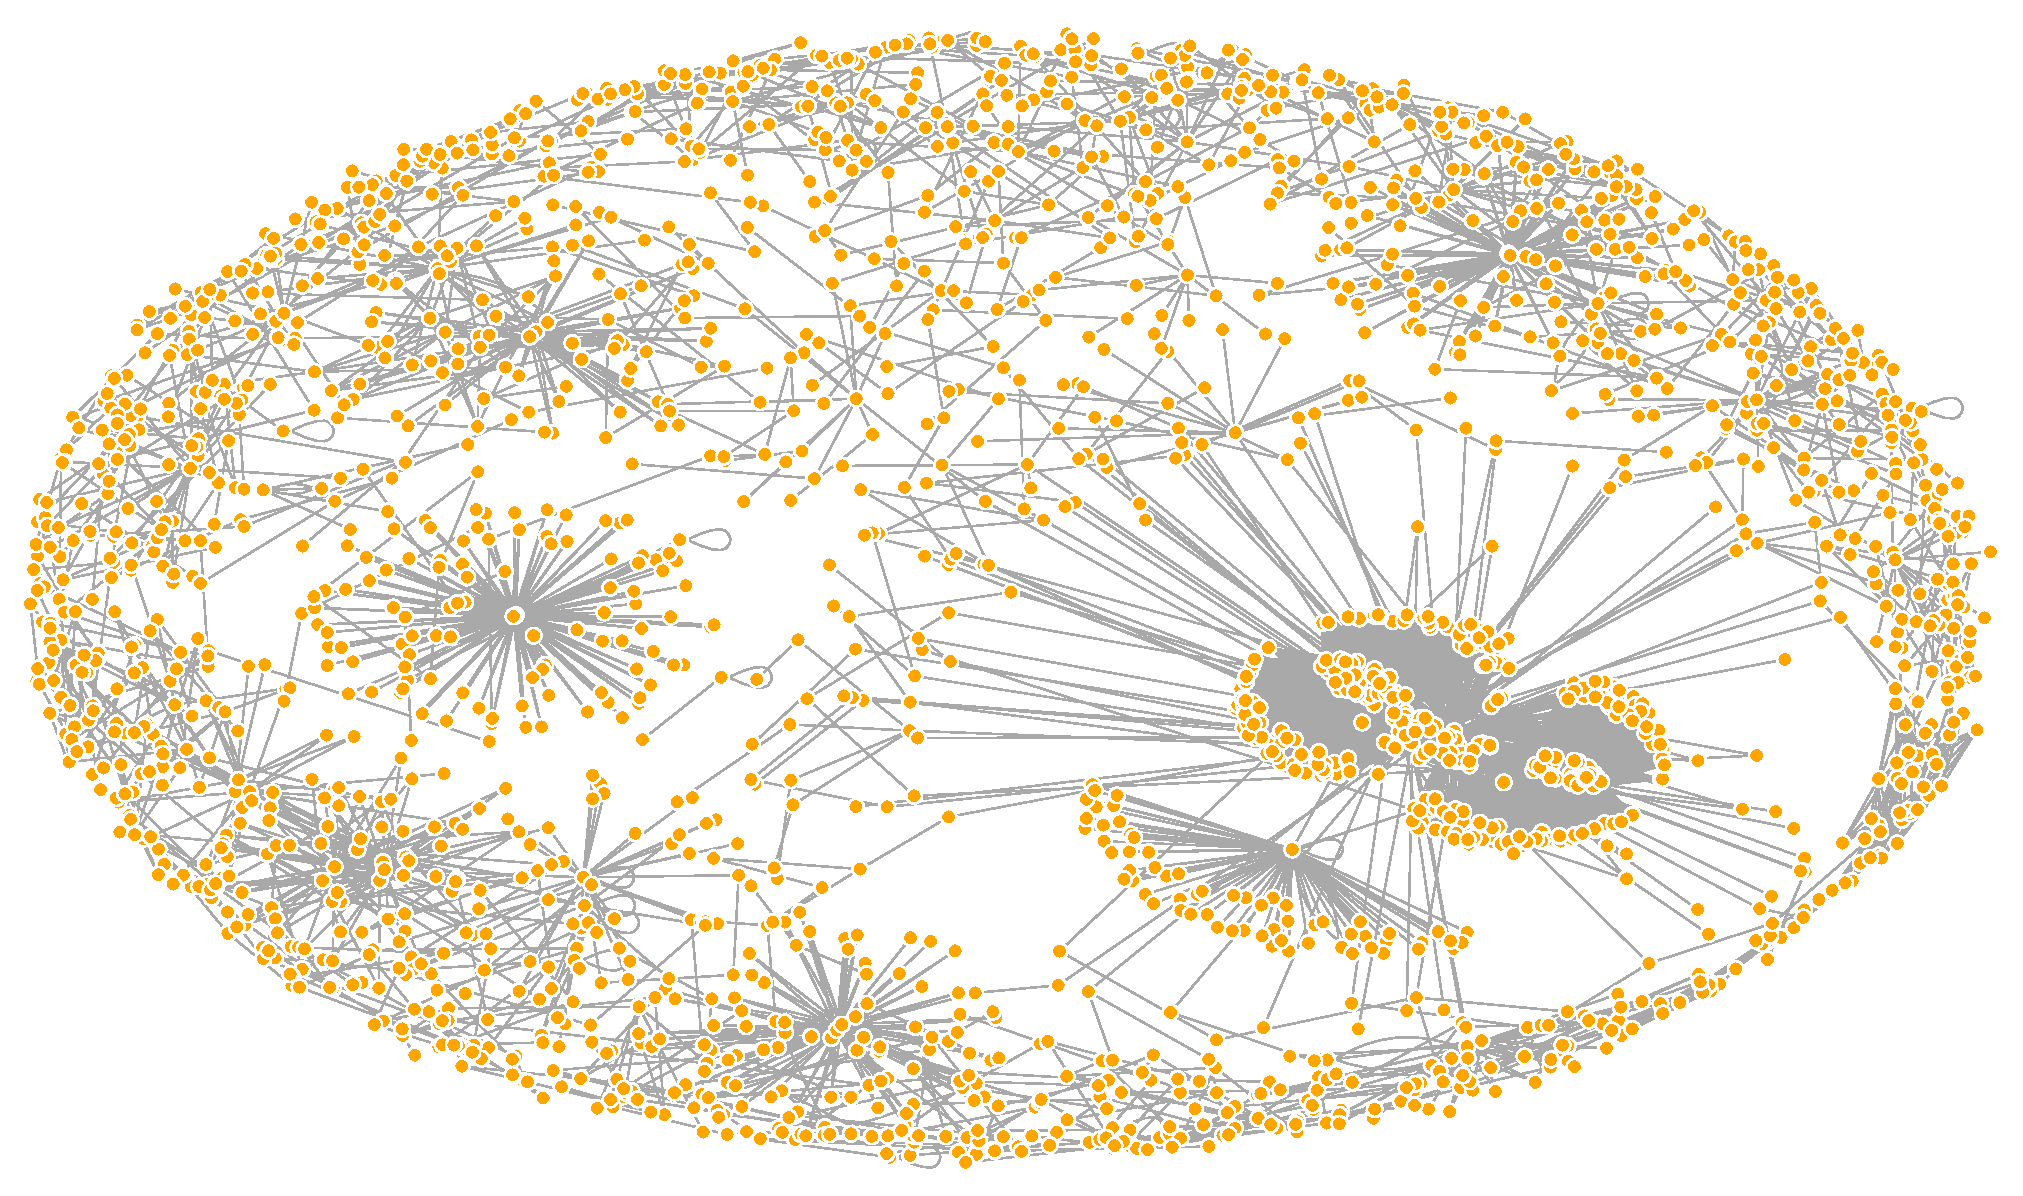
\includegraphics[width=3in]{Plots/address.eps}
\caption{\label{flow} Plot of the address graph constructed from half of the first November 2017 block.}
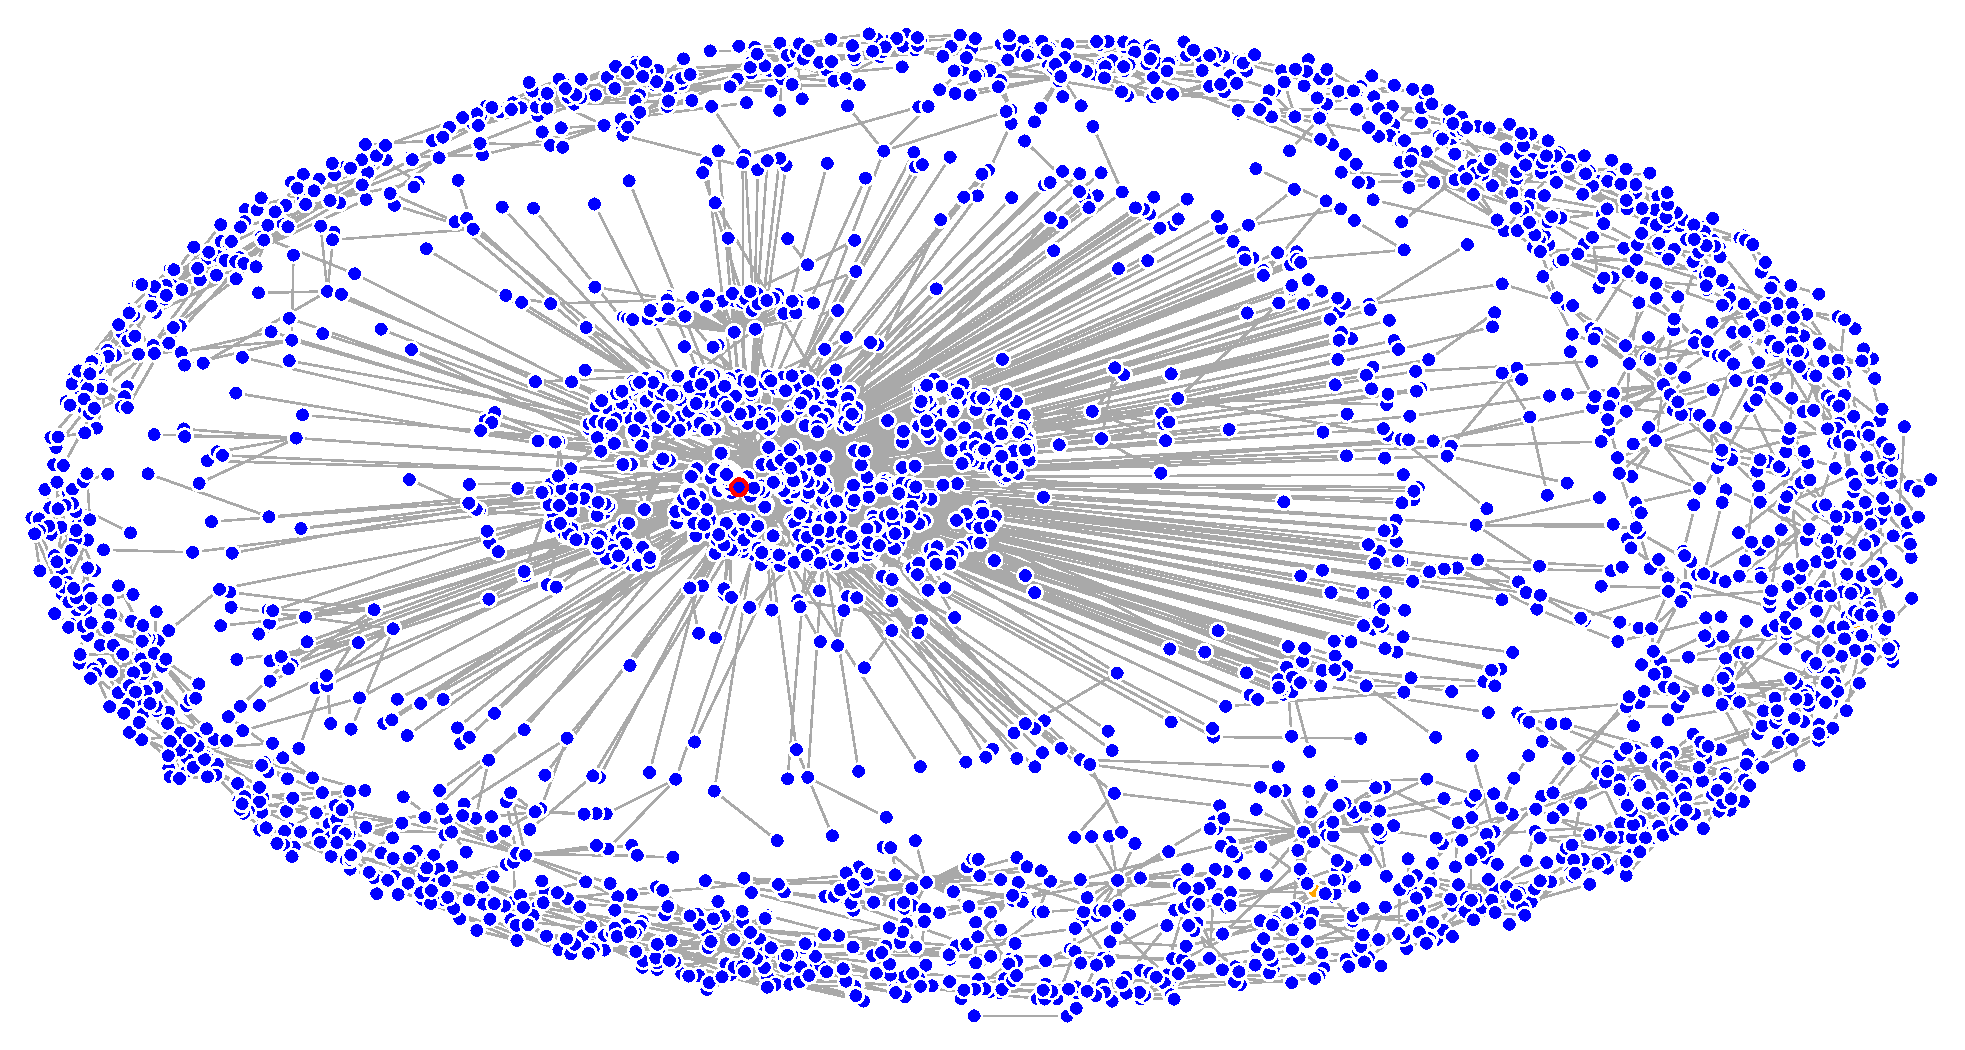
\includegraphics[width=3in]{Plots/transaction_november.eps}
\caption{\label{flow} Plot of the transaction graph constructed from half of the first November 2017 block.}
\end{figure}

\end{document}